\documentclass[10pt]{extarticle}
\title{}
\author{Avinash Iyer}
\date{}
\usepackage[shortlabels]{enumitem}

%font setup
%
\usepackage{newpxtext,eulerpx}

%paper setup
\usepackage{geometry}
\geometry{letterpaper, portrait, margin=1in}
\usepackage{fancyhdr}

%symbols
\usepackage{amsmath}
\usepackage{mathtools}
\usepackage{amssymb}
\usepackage{hyperref}
\usepackage{gensymb}

\usepackage[T1]{fontenc}
\usepackage[utf8]{inputenc}

%chemistry stuff
\usepackage[version=4]{mhchem}
\usepackage{chemfig}

%plotting
\usepackage{pgfplots}
\usepackage{tikz}
\tikzset{middleweight/.style={pos = 0.5, fill=white}}
\tikzset{weight/.style={pos = 0.5, fill = white}}
\tikzset{lateweight/.style={pos = 0.75, fill = white}}
\tikzset{earlyweight/.style={pos = 0.25, fill=white}}

%\usepackage{natbib}

%graphics stuff
\usepackage{graphicx}
\graphicspath{ {./images/} }

%code stuff
%when using minted, make sure to add the -shell-escape flag
%you can use lstlisting if you don't want to use minted
%\usepackage{minted}
%\usemintedstyle{pastie}
%\newminted[javacode]{java}{frame=lines,framesep=2mm,linenos=true,fontsize=\footnotesize,tabsize=3,autogobble,}
%\newminted[cppcode]{cpp}{frame=lines,framesep=2mm,linenos=true,fontsize=\footnotesize,tabsize=3,autogobble,}

\usepackage{listings}
\usepackage{color}
\definecolor{dkgreen}{rgb}{0,0.6,0}
\definecolor{gray}{rgb}{0.5,0.5,0.5}
\definecolor{mauve}{rgb}{0.58,0,0.82}

\lstset{frame=tb,
	language=Java,
	aboveskip=3mm,
	belowskip=3mm,
	showstringspaces=false,
	columns=flexible,
	basicstyle={\small\ttfamily},
	numbers=none,
	numberstyle=\tiny\color{gray},
	keywordstyle=\color{blue},
	commentstyle=\color{dkgreen},
	stringstyle=\color{mauve},
	breaklines=true,
	breakatwhitespace=true,
	tabsize=3
}
% text + color boxes
\usepackage{tcolorbox}
\tcbuselibrary{breakable}
\newtcolorbox{problem}[1]{colback = white, title = {#1}, breakable}
\newtcolorbox{solution}{colback = white, colframe = black!75!white, title = Solution, breakable}
%including PDFs
\usepackage{pdfpages}
\setlength{\parindent}{0pt}

\pagestyle{fancy}
\fancyhf{}
\rhead{Avinash Iyer}
\lhead{Homework Section 3.1, Individual}
\begin{document}
  \begin{problem}{3.1.1}
    Find a maximum matching in each graph below. Prove that it is a maximum matching by exhibiting an optimal solution to the dual problem (minimum vertex cover). Explain why this proves that the matching is optimal.
    \begin{center}
      Graph 1:\\
      \vspace{10pt}
      \begin{tikzpicture}
        \filldraw (0,0) circle (2pt)
              (1,0) circle (2pt)
              (2,0) circle (2pt)
              (3,0) circle (2pt)
              (4,0) circle (2pt)
              (0,1) circle (2pt)
              (1,1) circle (2pt)
              (2,1) circle (2pt)
              (3,1) circle (2pt);
        \draw (0,0) -- (2,1);
        \draw (1,0) -- (2,1);
        \draw (2,1) -- (2,0);
        \draw (1,0) -- (3,1);
        \draw (3,1) -- (2,0);
        \draw (3,0) -- (3,1);
        \draw (3,1) -- (4,0);
        \draw (0,1) -- (2,0);
        \draw (1,1) -- (2,0);
        \draw (2,1) -- (4,0);
      \end{tikzpicture}\\
      \vspace{20pt}
      Graph 2:\\
      \vspace{10pt}
      \begin{tikzpicture}
        \filldraw (0,0) circle (2pt)
                  (1,0) circle (2pt)
                  (2,0) circle (2pt)
                  (3,0) circle (2pt)
                  (4,0) circle (2pt);
        \filldraw (0,1) circle (2pt)
                  (1,1) circle (2pt)
                  (2,1) circle (2pt)
                  (3,1) circle (2pt)
                  (4,1) circle (2pt);
        \draw (0,1) -- (1,0);
        \draw (0,1) -- (2,0);
        \draw (1,1) -- (2,0);
        \draw (2,1) -- (1,0);
        \draw (3,1) -- (0,0);
        \draw (3,1) -- (2,0);
        \draw (3,1) -- (3,0);
        \draw (3,1) -- (4,0);
        \draw (4,1) -- (1,0);
        \draw (4,1) -- (2,0);
      \end{tikzpicture}\\
      \vspace{20pt}
      Graph 3:\\
      \vspace{10pt}
      \begin{tikzpicture}
        \filldraw (0,0) circle (2pt)
                  (1,0) circle (2pt)
                  (2,0) circle (2pt)
                  (3,0) circle (2pt)
                  (4,0) circle (2pt);
        \filldraw (0,1) circle (2pt)
                  (1,1) circle (2pt)
                  (2,1) circle (2pt)
                  (3,1) circle (2pt)
                  (4,1) circle (2pt);

        \draw (0,1) -- (1,0);
        \draw (0,1) -- (3,0);

        \draw (1,1) -- (0,0);
        \draw (1,1) -- (1,0);
        \draw (1,1) -- (2,0);
        \draw (1,1) -- (3,0);

        \draw (2,1) -- (1,0);
        \draw (2,1) -- (3,0);

        \draw (3,1) -- (0,0);
        \draw (3,1) -- (1,0);
        \draw (3,1) -- (3,0);
        \draw (3,1) -- (4,0);

        \draw (4,1) -- (1,0);
        \draw (4,1) -- (3,0);
      \end{tikzpicture}
    \end{center}
    \tcblower
    \begin{center}
      Graph 1:\\
      \vspace{10pt}
      \begin{tikzpicture}
        \filldraw (0,0) circle (2pt)
              (1,0) circle (2pt)
              (2,0) circle (2pt)
              (3,0) circle (2pt)
              (4,0) circle (2pt)
              (0,1) circle (2pt)
              (1,1) circle (2pt)
              (2,1) circle (2pt)
              (3,1) circle (2pt);
        \draw[very thick] (0,0) -- (2,1);
        \draw (1,0) -- (2,1);
        \draw (2,1) -- (2,0);
        \draw (1,0) -- (3,1);
        \draw (3,1) -- (2,0);
        \draw[very thick] (3,0) -- (3,1);
        \draw (3,1) -- (4,0);
        \draw[very thick] (0,1) -- (2,0);
        \draw (1,1) -- (2,0);
        \draw (2,1) -- (4,0);
      \end{tikzpicture}\\
      \vspace{10pt}
      \begin{tikzpicture}
        \filldraw (0,0) circle (2pt)
              (1,0) circle (2pt)
              (2,0) circle (2pt)
              (3,0) circle (2pt)
              (4,0) circle (2pt)
              (0,1) circle (2pt)
              (1,1) circle (2pt)
              (2,1) circle (2pt)
              (3,1) circle (2pt);
        \draw (2,1) circle (4pt)
              (2,0) circle (4pt)
              (3,1) circle (4pt);
        \draw (0,0) -- (2,1);
        \draw (1,0) -- (2,1);
        \draw (2,1) -- (2,0);
        \draw (1,0) -- (3,1);
        \draw (3,1) -- (2,0);
        \draw (3,0) -- (3,1);
        \draw (3,1) -- (4,0);
        \draw (0,1) -- (2,0);
        \draw (1,1) -- (2,0);
        \draw (2,1) -- (4,0);
      \end{tikzpicture}\\
      \vspace{20pt}
      Graph 2: \\
      \vspace{10pt}
      \begin{tikzpicture}
        \filldraw (0,0) circle (2pt)
                  (1,0) circle (2pt)
                  (2,0) circle (2pt)
                  (3,0) circle (2pt)
                  (4,0) circle (2pt);
        \filldraw (0,1) circle (2pt)
                  (1,1) circle (2pt)
                  (2,1) circle (2pt)
                  (3,1) circle (2pt)
                  (4,1) circle (2pt);
        \draw[very thick] (0,1) -- (1,0);
        \draw (0,1) -- (2,0);
        \draw (1,1) -- (2,0);
        \draw (2,1) -- (1,0);
        \draw[very thick] (3,1) -- (0,0);
        \draw (3,1) -- (2,0);
        \draw (3,1) -- (3,0);
        \draw (3,1) -- (4,0);
        \draw (4,1) -- (1,0);
        \draw[very thick] (4,1) -- (2,0);
      \end{tikzpicture}\\
      \vspace{10pt}
      \begin{tikzpicture}
        \filldraw (0,0) circle (2pt)
                  (1,0) circle (2pt)
                  (2,0) circle (2pt)
                  (3,0) circle (2pt)
                  (4,0) circle (2pt);
        \filldraw (0,1) circle (2pt)
                  (1,1) circle (2pt)
                  (2,1) circle (2pt)
                  (3,1) circle (2pt)
                  (4,1) circle (2pt);
        \draw (3,1) circle (4pt)
              (2,0) circle (4pt)
              (1,1) circle (4pt);
        \draw (0,1) -- (1,0);
        \draw (0,1) -- (2,0);
        \draw (1,1) -- (2,0);
        \draw (2,1) -- (1,0);
        \draw (3,1) -- (0,0);
        \draw (3,1) -- (2,0);
        \draw (3,1) -- (3,0);
        \draw (3,1) -- (4,0);
        \draw (4,1) -- (1,0);
        \draw (4,1) -- (2,0);
      \end{tikzpicture}\\
      \vspace{20pt}
      Graph 3:\\
      \vspace{10pt}
      \begin{tikzpicture}
        \filldraw (0,0) circle (2pt)
                  (1,0) circle (2pt)
                  (2,0) circle (2pt)
                  (3,0) circle (2pt)
                  (4,0) circle (2pt);
        \filldraw (0,1) circle (2pt)
                  (1,1) circle (2pt)
                  (2,1) circle (2pt)
                  (3,1) circle (2pt)
                  (4,1) circle (2pt);

        \draw[very thick] (0,1) -- (1,0);
        \draw (0,1) -- (3,0);

        \draw[very thick] (1,1) -- (0,0);
        \draw (1,1) -- (1,0);
        \draw (1,1) -- (2,0);
        \draw (1,1) -- (3,0);

        \draw (2,1) -- (1,0);
        \draw[very thick] (2,1) -- (3,0);

        \draw (3,1) -- (0,0);
        \draw (3,1) -- (1,0);
        \draw (3,1) -- (3,0);
        \draw[very thick] (3,1) -- (4,0);

        \draw (4,1) -- (1,0);
        \draw (4,1) -- (3,0);
      \end{tikzpicture}\\
      \vspace{10pt}
      \begin{tikzpicture}
        \filldraw (0,0) circle (2pt)
                  (1,0) circle (2pt)
                  (2,0) circle (2pt)
                  (3,0) circle (2pt)
                  (4,0) circle (2pt);
        \filldraw (0,1) circle (2pt)
                  (1,1) circle (2pt)
                  (2,1) circle (2pt)
                  (3,1) circle (2pt)
                  (4,1) circle (2pt);
        \draw (1,1) circle (4pt)
              (3,0) circle (4pt)
              (1,0) circle (4pt)
              (3,1) circle (4pt);

        \draw (0,1) -- (1,0);
        \draw (0,1) -- (3,0);

        \draw (1,1) -- (0,0);
        \draw (1,1) -- (1,0);
        \draw (1,1) -- (2,0);
        \draw (1,1) -- (3,0);

        \draw (2,1) -- (1,0);
        \draw (2,1) -- (3,0);

        \draw (3,1) -- (0,0);
        \draw (3,1) -- (1,0);
        \draw (3,1) -- (3,0);
        \draw (3,1) -- (4,0);

        \draw (4,1) -- (1,0);
        \draw (4,1) -- (3,0);
      \end{tikzpicture}
    \end{center}
    In all of these cases, we have solved the dual problem and found that the size of the minimum vertex cover is equal to the size of the maximum matching. Because all of these graphs are bipartite, we know that $\alpha'(G) = \beta(G)$.
  \end{problem}
  \begin{problem}{3.1.2}
    Determine the minimum size of a maximal matching in $C_n$.
    \tcblower
    The minimum size of a maximal matching in $C_n$ is $\left\lceil \frac{n}{3}\right\rceil$.\\
    \begin{description}[font=\normalfont\scshape]
      \item[Base Case] For $n = 3$, the minimum size of a maximal matching is $1$, and in $n =4$, the minimum size of a maximal matching is $2$, which are $\left\lceil \frac{n}{3}\right\rceil$ for $n = 3$ and $n=4$ respectively.
      \item[Inductive Step] In $C_k$, we assume that the minimum size of a maximal matching is $\left\lceil \frac{k}{3} \right\rceil$. For $k+1$, we have the following cases that we will prove:
        \begin{description}[font=\normalfont]
          \item[$k+1 \equiv 1$ mod $3$:] If $k+1$ is congruent to $1$ modulo $3$, then $C_k$ is of the form $C_{3n}$, with a minimum-size maximal matching of $\left\lceil \frac{k}{3}\right\rceil$. The edge pattern of a maximal matching $M$ in a $3n$-gon is $m_1, e_1, e_2, m_2,e_3,e_4,\dots$ for $m_i\in M$ and $e_i \in E(C_k) - M$. Insertion of an edge $e$ (and its requisite vertices) to create $C_{k+1}$ would yield an edge pattern of $m_1,e_1,e,e_2,\dots$, meaning that $M'$ would need to include $e$ to be a maximal matching. Therefore $|M'| = |M| + 1 = \left\lceil \frac{k+1}{3} \right\rceil$.
          \item[$k+1\equiv 2$ mod $3$:] If $k+1$ is congruent to $2$ modulo $3$, then $k$ is congruent to $1$ modulo $3$, meaning that by our previous construction, there exists the pattern $m_1,e_1,m_2,e_2,m_3,\dots$. Therefore, we can insert an edge $e$ to construct our $C_{k+1}$ such that the edge pattern is $m_1,e_1,e,m_2,\dots$, meaning that the size of our $M'$ does not change. Therefore $|M'| = |M| = \left\lceil \frac{k+1}{3}\right\rceil$.
          \item[$k+1\equiv 0$ mod 3:] If $k+1$ is congruent to $0$ modulo $3$, then $k$ is congruent to $2$ modulo $3$, meaning by our previous result, there must be one edge pattern of $m_1,e_1,m_2,\dots$ for $m_i\in M$ and $e_i\in E(C_k) - M$. So, we are able to insert $e$ to create $C_{k+1}$ as $m_1,e_1,e,m_2$ as with the previous case, meaning $|M'| = |M| = \left\lceil \frac{k+1}{3}\right\rceil$.
        \end{description}
    \end{description}
  \end{problem}
  \begin{problem}{3.1.5}
    Prove that $\alpha(G) \geq \frac{n(G)}{\Delta(G)+1}$ for every graph $G$.
    \tcblower
    \begin{align*}
      \alpha(G) + \beta(G) &= n(G) \\
      \alpha(G) &= n(G) - \beta(G) \\
      \alpha(G) &\geq n(G) - \alpha(G)\Delta(G) \tag*{$\alpha(G)\Delta(G) = \max \beta(G)$} \\
      \alpha(G) &\geq \frac{n(G)}{\Delta(G) + 1}
    \end{align*}
  \end{problem}
  \begin{problem}{3.1.9}
    Prove that every maximal matching in a graph $G$ has at least $\alpha'(G)/2$ edges.
    \tcblower
    Let $M$ be a maximal matching with fewer than $\alpha'(G)/2$ edges. Since $M$ is maximal, we are assuming that every vertex in $G$ is either in $M$ or is adjacent to a vertex in $M$. Since $M$ is a maximal matching that is \textit{not} a maximum matching, then there must be an $M$-augmenting path.\\

    Let $v$ be the start of this $M$-augmenting path, and let $w$ be its final vertex. Because $v$ and $w$ cannot have any other edges incident on them, we must assume that $\alpha'(G) = |M| + 1$, as we can exchange the matchings within the $M$-augmenting path to get a maximum matching. However, because $|M| < \alpha'(G)/2$, we must get that $\alpha'(G) < 1 + \alpha'(G)/2$, or that $\alpha'(G) < 2$. However, $\alpha'(G)/2$ must be an integer, meaning that the original assumption (that $M$ is a maximal matching) must be false.
  \end{problem}
  \begin{problem}{3.1.28}
    Exhibit a perfect matching in the graph below or give a short proof that it has none. 
    \begin{center}
      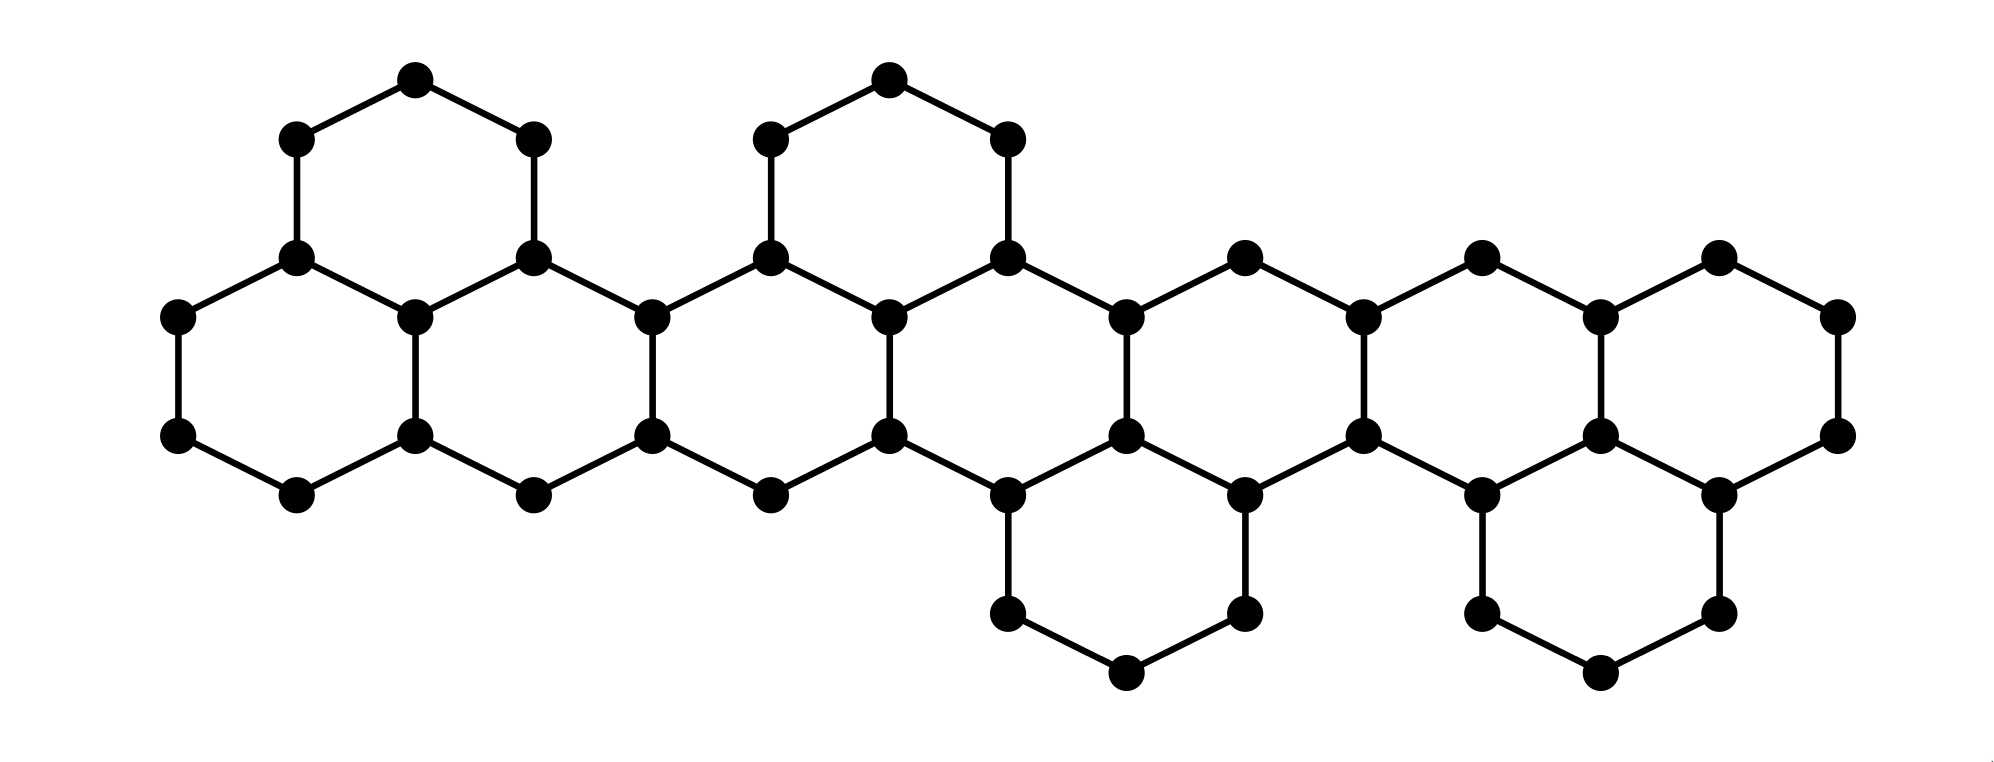
\includegraphics[width=10cm]{3_1_28_question}
    \end{center}
    \tcblower
    The minimum edge cover is as follows, and is of size $22$, meaning that the maximum matching is of size $20$ (as this graph is bipartite), which is not a perfect matching.
    \begin{center}
      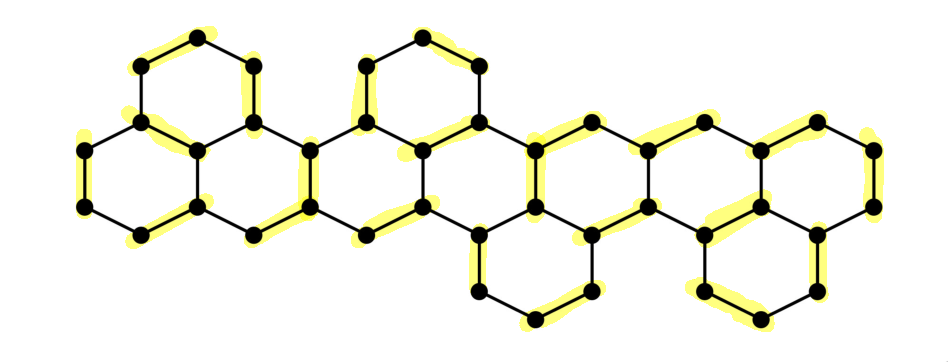
\includegraphics[width=10cm]{3_1_28_ans.pdf}
    \end{center}
  \end{problem}
\end{document}
